Calibration is fundamental to ensuring the accuracy and reliability of an automated robotic workcell. The calibration process takes exactly 98 seconds for the robot. Proper calibration ensures that the robot operate with high accuracy, thus reducing variability in the bent sheet metal part.

Figure \ref{fig:calibration-parameters} shows the calibration parameters after an automatic calibration. The field of view is 100\% with a resolution of 0.1564 mm/px.

\begin{figure}[h]
    \centering
    \begin{subfigure}{0.48\textwidth}
        \centering
        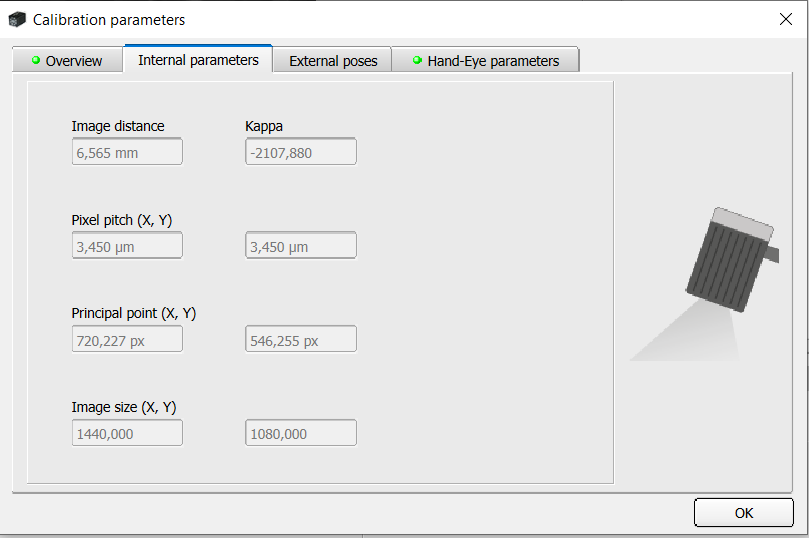
\includegraphics[width=\textwidth]{figures/001calibration/internal_parameters.PNG}
        \caption{Internal parameters}
        \label{subfig:internal-parameters}
    \end{subfigure}\hspace{0cm}
    \begin{subfigure}{0.48\textwidth}
        \centering
        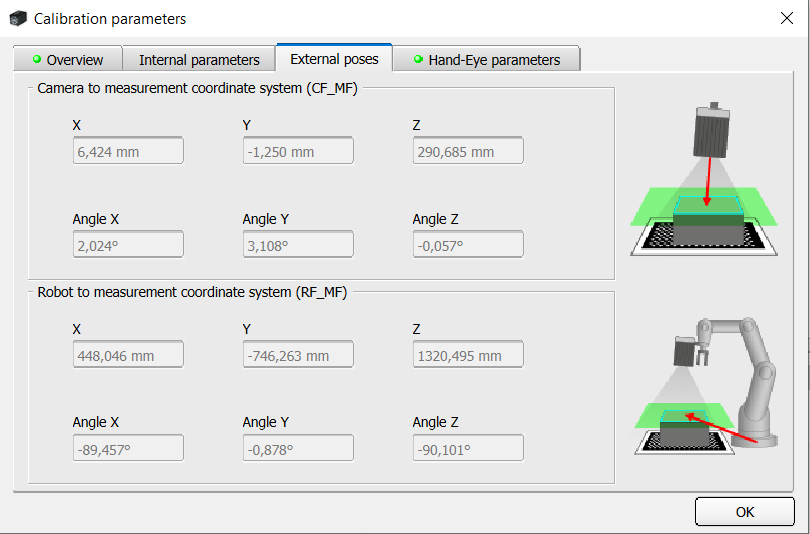
\includegraphics[width=\textwidth]{figures/001calibration/external_poses.PNG}
        \caption{External poses}
        \label{subfig:external-poses}
    \end{subfigure}
    \begin{subfigure}{0.48\textwidth}
        \centering
        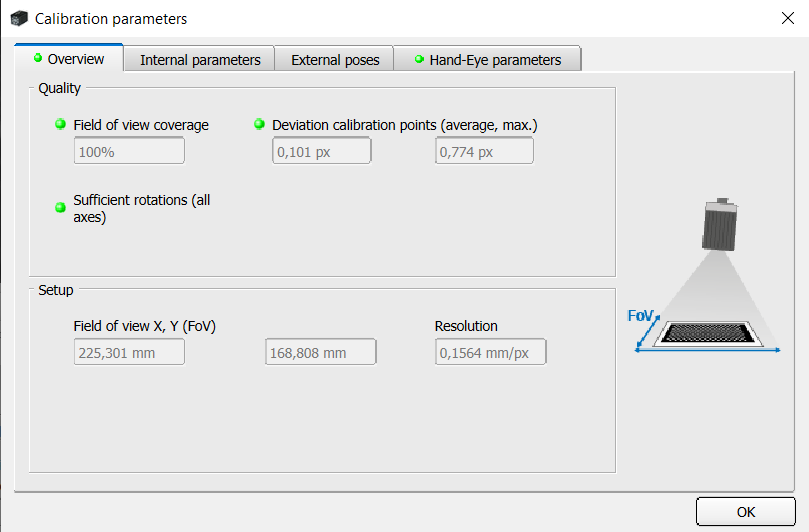
\includegraphics[width=\textwidth]{figures/001calibration/fov.PNG}
        \caption{Field of view}
        \label{subfig:fov}
    \end{subfigure}
    \begin{subfigure}{0.48\textwidth}
        \centering
        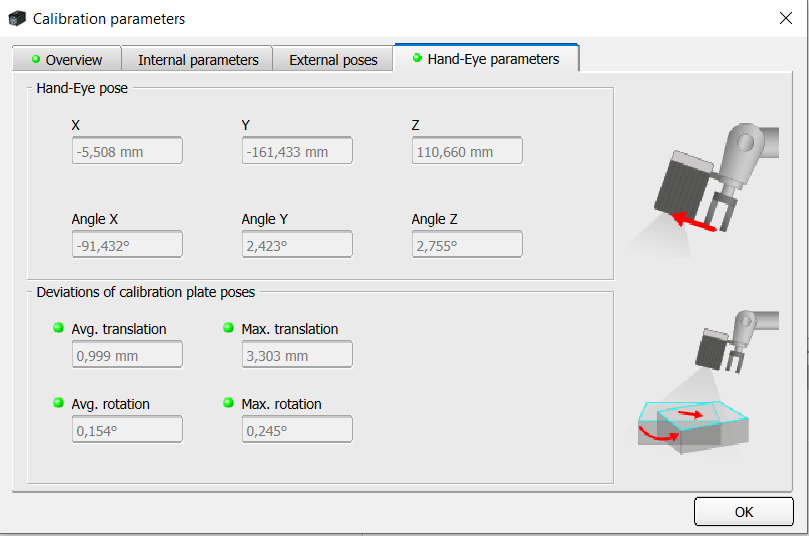
\includegraphics[width=\textwidth]{figures/001calibration/hand-eye_parameters.PNG}
        \caption{Hand-eye parameters}
        \label{subfig:hand-eye-parameters}
    \end{subfigure}
    \caption{Calibration parameters}
    \label{fig:calibration-parameters}
\end{figure}


By establishing rigorous calibration procedures, the automated robotic workcell can achieve optimal performance, ensuring that the bending process is executed with high precision and reliability.  The KR1410 robot only has a repeatability of 0.1 mm. After the TCP calibration, the bending process has a repeatability of 0.5 mm, which is still better than a human operator.
